\documentclass[tikz,border=12pt]{standalone}
% Shared visual language for standalone EMT block diagrams.
\usepackage{amsmath}
\usetikzlibrary{arrows.meta,backgrounds,calc,fit,positioning}

\tikzset{
    emt diagram/.style = {>={Stealth[length=2.4mm]}},
    line/.style        = {semithick, rounded corners=6pt},
    block/.style       = {draw, semithick, fill=white,
                          minimum height=1cm, minimum width=2.3cm},
    hblock/.style      = {block, minimum width=2.24cm, minimum height=1.3cm},
    vblock/.style      = {block, minimum width=1.3cm, minimum height=2.24cm},
    sum/.style         = {draw, semithick, fill=white, circle,
                          inner sep=2.6pt},
    signal/.style      = {circle, fill, inner sep=1.4pt,
                          label distance=3pt},
    sig/.style         = {font=\small},
    pm/.style          = {font=\scriptsize},
    wire jump/.style   = {line,
                          preaction={draw=white, line width=3pt,
                                     line cap=round}},
    enclosure/.style   = {draw, dashed, semithick, rounded corners=4pt},
    operator enclosure/.style = {enclosure, inner xsep=7mm, inner ysep=6mm}
}


\begin{document}
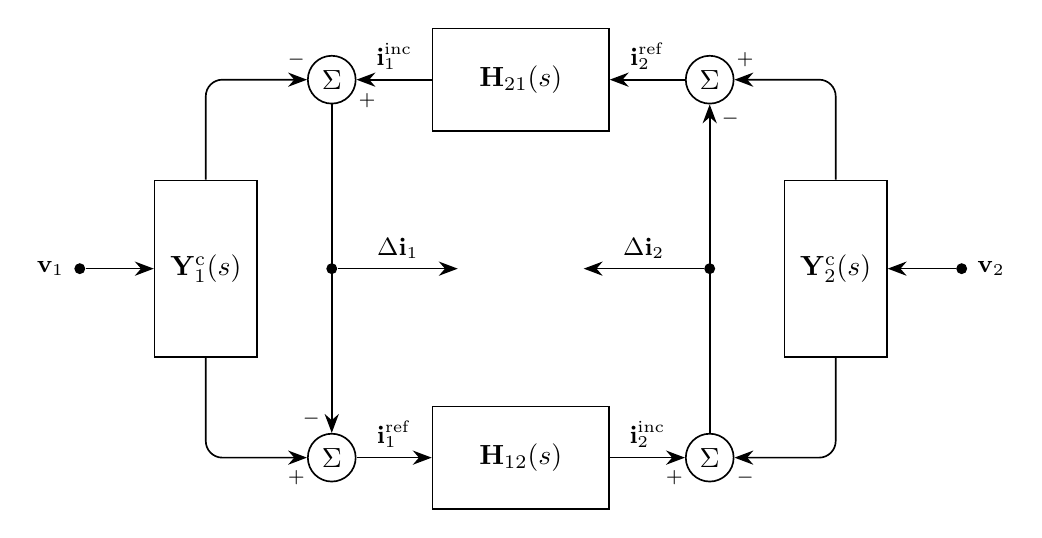
\begin{tikzpicture}[emt diagram]

% ================= Terminal 1 (left column) =================
\node[sum]   (kcl1)  at (-2.4,  2.4) {$\Sigma$};
\node[vblock] (Yc1)  at (-4.0,  0.0) {$\mathbf{Y}^{\mathrm{c}}_1(s)$};
\node[sum]   (wave1) at (-2.4, -2.4) {$\Sigma$};

\node[signal, label={[sig]left:$\mathbf{v}_1$}] (v1) at (-5.6, 0) {};

\draw[->, line] (Yc1.north) |- (kcl1.west);
\draw[->, line] (Yc1.south) |- (wave1.west);
\draw[->, line] (kcl1.south) -- (wave1.north);
\node[signal] (i1split) at (kcl1 |- v1) {};
\draw[->, line] (i1split) -- node[sig, above] {$\Delta\mathbf{i}_1$} ++(1.6,0);

\draw[->, line] (v1) -- (Yc1.west);

% ================= Terminal 2 (right column) =================
\node[sum]   (wave2) at (2.4,  2.4) {$\Sigma$};
\node[vblock] (Yc2)  at (4.0,  0.0) {$\mathbf{Y}^{\mathrm{c}}_2(s)$};
\node[sum]   (kcl2)  at (2.4, -2.4) {$\Sigma$};

\node[signal, label={[sig]right:$\mathbf{v}_2$}] (v2) at (5.6, 0) {};

\draw[->, line] (Yc2.north) |- (wave2.east);
\draw[->, line] (Yc2.south) |- (kcl2.east);
\draw[->, line] (kcl2.north) -- (wave2.south);
\node[signal] (i2split) at (kcl2 |- v2) {};
\draw[->, line] (i2split) -- node[sig, above] {$\Delta\mathbf{i}_2$} ++(-1.6,0);

\draw[->, line] (v2) -- (Yc2.east);

% ================= Propagation channels (straight rows) =================
% 1 -> 2 (lower row, left to right)
\node[hblock] (H12) at (0, -2.4) {$\mathbf{H}_{12}(s)$};
\draw[->, line] (wave1.east) -- node[sig, above] {$\mathbf{i}^{\mathrm{ref}}_1$} (H12.west);
\draw[->, line] (H12.east) -- node[sig, above] {$\mathbf{i}^{\mathrm{inc}}_2$} (kcl2.west);

% 2 -> 1 (upper row, right to left)
\node[hblock] (H21) at (0,  2.4) {$\mathbf{H}_{21}(s)$};
\draw[->, line] (wave2.west) -- node[sig, above] {$\mathbf{i}^{\mathrm{ref}}_2$} (H21.east);
\draw[->, line] (H21.west) -- node[sig, above] {$\mathbf{i}^{\mathrm{inc}}_1$} (kcl1.east);

% ================= Summation signs =================
\node[pm] at ($(kcl1)+(-0.45, 0.26)$) {$-$};   % Yc1 v1 subtracts
\node[pm] at ($(kcl1)+( 0.45,-0.26)$) {$+$};   % incident current adds
\node[pm] at ($(wave1)+(-0.45,-0.26)$) {$+$};  % Yc1 v1
\node[pm] at ($(wave1)+(-0.26, 0.50)$) {$-$};  % i1
\node[pm] at ($(kcl2)+( 0.45,-0.26)$) {$-$};   % Yc2 v2 subtracts
\node[pm] at ($(kcl2)+(-0.45,-0.26)$) {$+$};   % incident current adds
\node[pm] at ($(wave2)+( 0.45, 0.26)$) {$+$};  % Yc2 v2
\node[pm] at ($(wave2)+( 0.26,-0.50)$) {$-$};  % i2

\end{tikzpicture}
\end{document}
